\documentclass[border=10pt]{standalone}
\usepackage[svgnames]{xcolor}
\usepackage{amsmath}
\usepackage{pgfplots}
\pgfplotsset{compat=newest}
\usepackage[sfdefault]{FiraSans}
\usepackage{FiraMono}
\renewcommand*\familydefault{\sfdefault}
\begin{document}
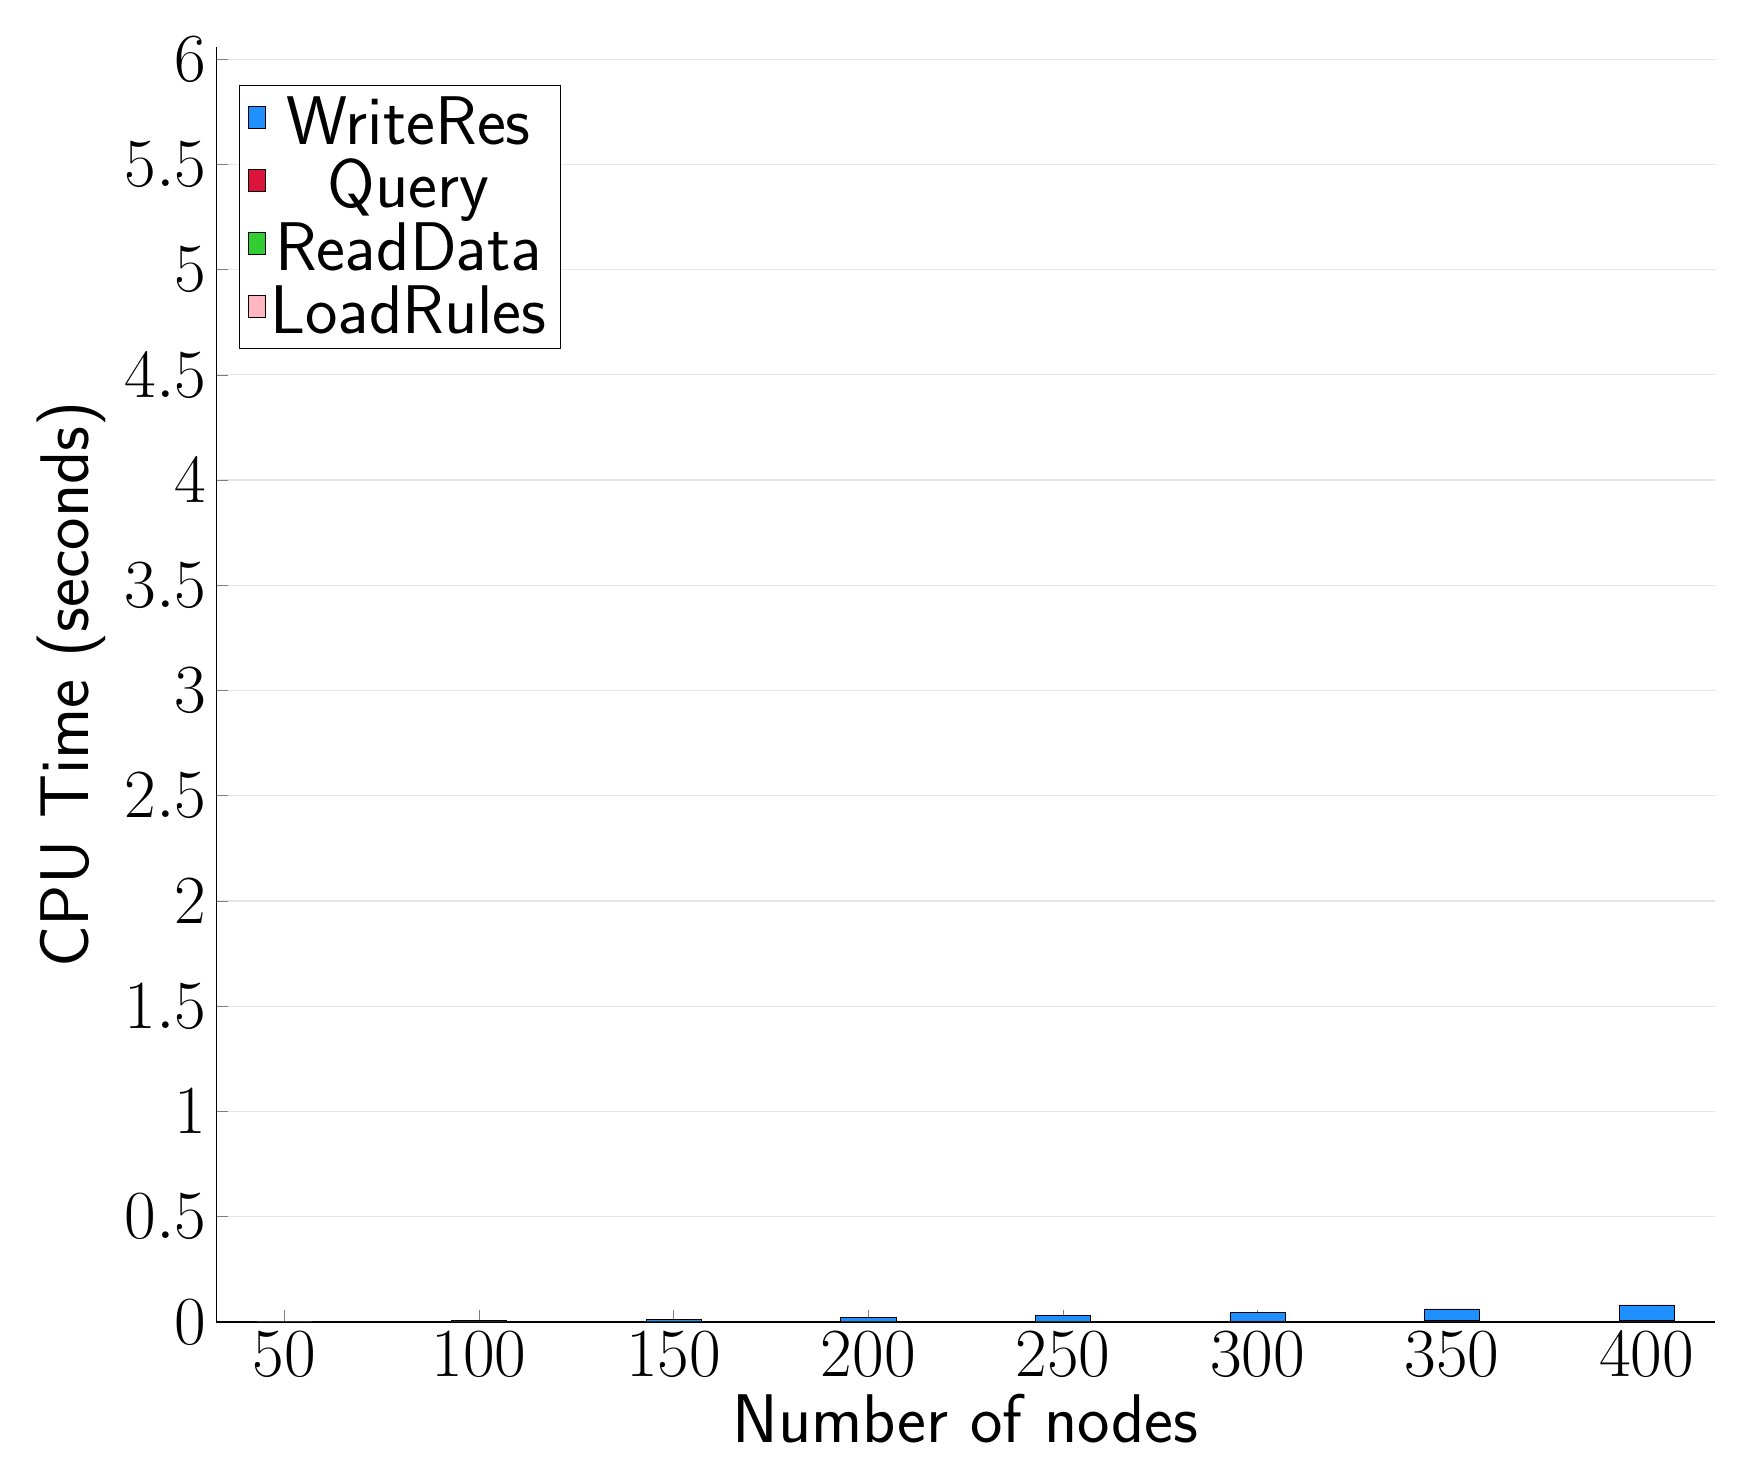
\begin{tikzpicture}
\begin{axis}[
   ybar stacked,
   width=1.7\textwidth,
   bar width=0.7cm,
   ymajorgrids, tick align=inside,
   major grid style={draw=gray!20},
   xtick=data,
   ymin=0, ymax=6.059334,
   axis x line*=bottom,
   axis y line*=left,
   enlarge x limits=0.05,
   legend style={
       at={(0.23, 0.97)},
       anchor=north east,
       legend columns=1,
       font=\Huge,
   },
   ylabel={CPU Time (seconds)},
   xlabel={Number of nodes},
   label style={font=\Huge},
   tick label style={font=\Huge},
]
\addlegendimage{fill=DodgerBlue, draw=black, line width=0.2pt}
\addlegendentry{WriteRes}
\addlegendimage{fill=Crimson, draw=black, line width=0.2pt}
\addlegendentry{Query}
\addlegendimage{fill=LimeGreen, draw=black, line width=0.2pt}
\addlegendentry{ReadData}
\addlegendimage{fill=LightPink, draw=black, line width=0.2pt}
\addlegendentry{LoadRules}
\addplot +[fill=LightPink, draw=black, line width=0.2pt] coordinates {
(50, 0.0006195000000000006)
(100, 0.0006214000000000003)
(150, 0.0006144)
(200, 0.0006048999999999999)
(250, 0.0006013999999999999)
(300, 0.0006062999999999999)
(350, 0.0005998000000000002)
(400, 0.0006214999999999994)
};
\addplot +[fill=LimeGreen, draw=black, line width=0.2pt] coordinates {
(50, 0.00018590000000000018)
(100, 0.00021870000000000033)
(150, 0.00026129999999999985)
(200, 0.00030829999999999985)
(250, 0.0003473)
(300, 0.0004097999999999998)
(350, 0.0004373000000000003)
(400, 0.0004980000000000007)
};
\addplot +[fill=Crimson, draw=black, line width=0.2pt] coordinates {
(50, 0.0001295999999999998)
(100, 0.00045109999999999996)
(150, 0.0009852000000000003)
(200, 0.0017645999999999998)
(250, 0.0026944000000000004)
(300, 0.0038774000000000005)
(350, 0.0052242)
(400, 0.0068619)
};
\addplot +[fill=DodgerBlue, draw=black, line width=0.2pt] coordinates {
(50, 0.0011511000000000004)
(100, 0.004515900000000001)
(150, 0.010451)
(200, 0.0184529)
(250, 0.0293155)
(300, 0.0411711)
(350, 0.056350899999999995)
(400, 0.073667)
};
\end{axis}
\end{tikzpicture}

\end{document}
